\section{Wirbelfrequenzzähler}
\subsection{Aufbau und Funktionsweise eines Wirbelfrequenzzählers}
In Abbildung \ref{fig:wirbelzaehler} ist der typische Aufbau eines Wirbelfrequenzzählers, auch Wirbeldurchflussmesser genannt, dargestellt. Im Wesentlichen besteht dieser aus einem Messrohr(4), in dem ein Staukörper(1) mit bestimmter Geometrie(5) eingelassen ist. Hinter diesem ist ein Wirbeldruckabnehmer (2) verbaut. Das erzeugte Signal wird von einer Auswertelektronik verarbeitet und dem Anwender ausgegeben.\autocite[vgl.][803\psqq]{Sensortechnik}
\begin{figure}[H]
   \centering
    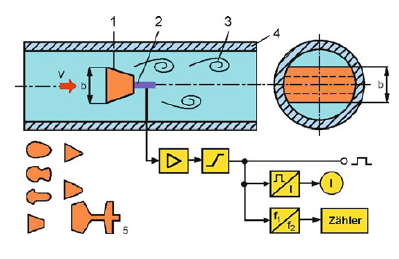
\includegraphics[scale=0.75]{Bilder/Wirbelzaehler.png}
    \caption[Aufbau eines Wirbeldurchflussmessers]{Aufbau eines Wirbeldurchflussmessers\footnotemark}
    \label{fig:wirbelzaehler}
\end{figure}
\footnotetext{\cite[][291]{Sensoren}}
Das Messprinzip beruht auf der K\'{a}rm\'{a}n`schen Wirbelstraße. Durch den Staukörper entstehen bei strömenden Medien sich periodisch abwechselnde Wirbel. Diese erzeugen hinter der Staugeometrie einen Unterdruck, der ebenso periodisch variiert. Die Druckschwankung bringt den Wirbeldruckabnehmer in Schwingung. Mithilfe eines Sensorelements wird die Frequenz $f$ der Schwingung in ein elektrisch auswertbares Signal umgewandelt. Dies kann mechanisch, akustisch oder optisch erfolgen.\autocite[vgl.][S. 803]{Sensortechnik}\\
Die mathematische Ermittlung der Strömungsgeschwindigkeit $u$ beruht auf der Proportionalität zur Ablösefrequenz $f$: 
\begin{eqnarray}\label{for:f}
    f &=& K_1 \cdot u \\
    mit: \quad K_1 &=& Proportionalit\ddot{a}tsfaktor \nonumber
\end{eqnarray}
Desweiteren gilt für den Volumenstrom $Q_v$ folgende Abhängigkeit:
\begin{eqnarray}
    Q_v &=& u \cdot A \\
    mit: \quad A &=& Messrohrquerschnitt \nonumber
\end{eqnarray}
Der Messrohrquerschnitt $A$ ist bei dem jeweiligen Wirbelfrequenzzähler konstant, sodass sich für den Kalibrierfaktor $K$ eines Wirbelzählers folgender Zusammenhang besteht:
\begin{eqnarray}
    f &=& K \cdot Q_v
\end{eqnarray}
Somit kann der Volumenstrom direkt aus der gemessenen Ablösefrequenz $f$ und des Kalibrierfaktors $K$ berechnet werden. Setzt man Formel (\ref{for:f}) in die Formel (\ref{for:Sr}), Seite \pageref{for:Sr} ein, erhält man für den Proportionalitätsfaktor $K_1$:
\begin{eqnarray}
    S_r &=& K_1 \cdot d
\end{eqnarray}
Da die Strouhal-Zahl $Sr$ in einem bestimmten Bereich der Reynolds-Zahl $Re$ nahezu konstant ist, kann der Proportionalitätsfaktor $K_1$ und damit auch der Kalibrierfaktor $K$ bestimmt werden. In der Regel wird dieser jedoch nicht berechnet, sondern direkt vom Hersteller kalibriert.\autocite[vgl.][S. 806 \psq]{Sensortechnik}

\subsection{KROHNE OPTISWIRL 4200}
Der $OPTISWIRL \: 4200$ der Firma  $KROHNE$ arbeitet nach dem Prinzip der K\'{a}rm\'{a}n`schen Wirbelstraße. Die Sensoreinheit zur Erfassung der Wirbelfrequenz ist im Benutzerhandbuch nicht näher ausgeführt, jedoch sind im Kapitel \textit{\glqq Statusmeldungen und Diagnose-Informationen\grqq{}}, Seite 96 des Benutzerhandbuches unter der Ereignisgruppe \textit{\glqq Sensor\grqq{}} Fehlermeldungen beschrieben, die sich auf ein Piezoelement beziehen. Somit kann davon ausgegangen werden, dass die primäre Messgröße (Anzahl der abgelösten Wirbel) mithilfe eines Piezoelements erfasst wird. Die periodische Druckschwankung wirkt auf das Piezoelement und erzeugt ein periodisch schwankendes, elektrisches Potenzial, welches der Wirbelfrequenz entspricht. Als sekundäre Messgröße gibt der Hersteller zusätzlich den Betriebs-, Norm-, Volumen- und -Massedurchfluss an. Weiterhin kann die Temperatur und optional der Druck erfasst werden. Den $OPTISWIRL \: 4200$ gibt es in verschiedenen Ausführungen, die sich nach dem jeweiligen Einsatzzweck richten. \autocite[vgl.][96, 107 \psq]{Optiswirl}

\subsection{Endress+Hauser Prowirl 200}
Die Firma \textit{Endress+Hauser} stellt ebenso ein Wirbeldurchflussmessgerät her, welches das Prinzip der K\'{a}rm\'{a}n`schen Wirbelstraße nutzt. Die Wirbelfrequenz wird beim  $Proline \: Prowirl \: F \: 200$ mithilfe eines kapazitiven Sensors in ein elektrisch auswertbares Signal umgewandelt. Vereinfacht dargestellt, besteht dieser Sensor aus zwei parallel gegenüberliegenden Kondensatorplatten. Der Abstand zwischen den Kondensatorplatten kann durch äußere Einwirkungen variieren. Dadurch verändert sich die Kapazität des Kondensators, die messtechnisch erfasst und ausgewertet wird. Zusätzliche Messgrößen können wie beim $OPTISWIRL \: 4200$ ebenso erfasst werden. Als Alleinstellungsmerkmal bewirbt \textit{Endress+Hauser} den $Proline \: Prowirl \: F \: 200$ mit einer integrierten Nassdampferkennung. Die Kalibrierung des Proportionalitätsfaktors $K$ ist für nicht abrasive Medien auf \textit{\glqq Lebenszeit\grqq{}} angegeben, da der Sensor keinem Langzeit- oder Nullpunktdrift unterliegt. In abrasiven Medien kann sich jedoch die Geometrie des Staukörpers geringfügig ändern. Dies verändert den $K-Wert$, sodass eine Neukalibrierung nach bestimmten Zeitabständen erforderlich ist.\autocites[vgl.][476 \psq]{Sensortechnik}[vgl.][4 \psq]{Prowirl}

\subsection{Gegenüberstellung der beiden Messgeräte}
In Tabelle \ref{tab:uebersicht}, Seite \pageref{tab:uebersicht} sind die wichtigsten technischen Eigenschaften der beiden Hersteller gegenübergestellt. Als Nennweite wurde $DN25$  gewählt. Diese Kenngröße ist ein typisches Merkmal von Rohrleitungssystemen. Sie folgt der $DIN \: EN \: ISO \: 6708$ und stellt sicher, dass zueinander gehörende Bauteile bei Rohrleitungssystemen passgenau sind. Die Innendurchmesser sind annähernd gleich. Dadurch ist der Vergleich und die Leistungsbeurteilung der einzelnen Messgeräte möglich.\autocite[vgl.][399]{technischesZeichnen}\\
Die Einsatztemperatur ist für beide Geräte annähernd gleich. Trotzdem ist der $Prowirl \: F \: 200$ für höhere Messstofftemperaturen geeignet. Bei der Durchflussgeschwindigkeit weist der $OPTISWIRL$ ein kleineres Spektrum auf als das Konkurenzprodukt. Für geringere Durchflussgeschwindigkeiten von Gasen und Dämpfen ist der $Prowirl \: F \: 200$ aufgrund der minimalen Fließgeschwindigkeit von $0,7 \frac{m}{s}$ geeignet. Jedoch liegt die maximale Durchflussgeschwindigkeit beim $Prowirl \: F \: 200$ unter dem Wert des zweiten Produkts. Der maximale Messdruck sowie die Genauigkeit der ermittelten Messwerte ist bei beiden gleich. Die Versorgungsspannung kann beim $Prowirl \: F \: 200$ um $5V$ höher bei maximal $35V$ liegen. Beide Messgeräte unterstützen die gängigen Kommuniktationsschnittstellen für den Industriegebrauch, der $Prowirl \: F \: 200$ verfügt zusätzlich über eine von \textit{Endress+Hauser} entwickelte Serviceschnittstelle. Für den $OPTISWIRL \: 4200$ lässt sich dazu im Benutzerhandbuch keine Information finden.\autocites[vgl.][9 \psqq]{Prowirl}[vgl.][108 \psqq]{Optiswirl}
\input{Tabellen/gegenueberstellung}
Die Preise für die jeweiligen Wirbelfrequenzzähler sind öffentlich nicht einsehbar. Gebrauchte Geräte auf dem freien Markt lassen allerdings die Schlussfolgerung zu, dass das Messgerät der Firma \textit{Endress+Hauser} deutlich höher ausfällt, als das Modell des Konkurrenten. Welches Messgerät besser ist, lässt sich pauschal jedoch nicht feststellen, da der Einsatzzweck, das verwendete Medium und der Kostenrahmen in der Regel die entscheidenden Faktoren sind.\autocites[vgl.][]{KostenOptiswirl}[vgl.][]{KostenProwirl}